\documentclass[]{ximera}
%handout:  for handout version with no solutions or instructor notes
%handout,instructornotes:  for instructor version with just problems and notes, no solutions
%noinstructornotes:  shows only problem and solutions

%% handout
%% space
%% newpage
%% numbers
%% nooutcomes

%I added the commands here so that I would't have to keep looking them up
%\newcommand{\RR}{\mathbb R}
%\renewcommand{\d}{\,d}
%\newcommand{\dd}[2][]{\frac{d #1}{d #2}}
%\renewcommand{\l}{\ell}
%\newcommand{\ddx}{\frac{d}{dx}}
%\everymath{\displaystyle}
%\newcommand{\dfn}{\textbf}
%\newcommand{\eval}[1]{\bigg[ #1 \bigg]}

%\begin{image}
%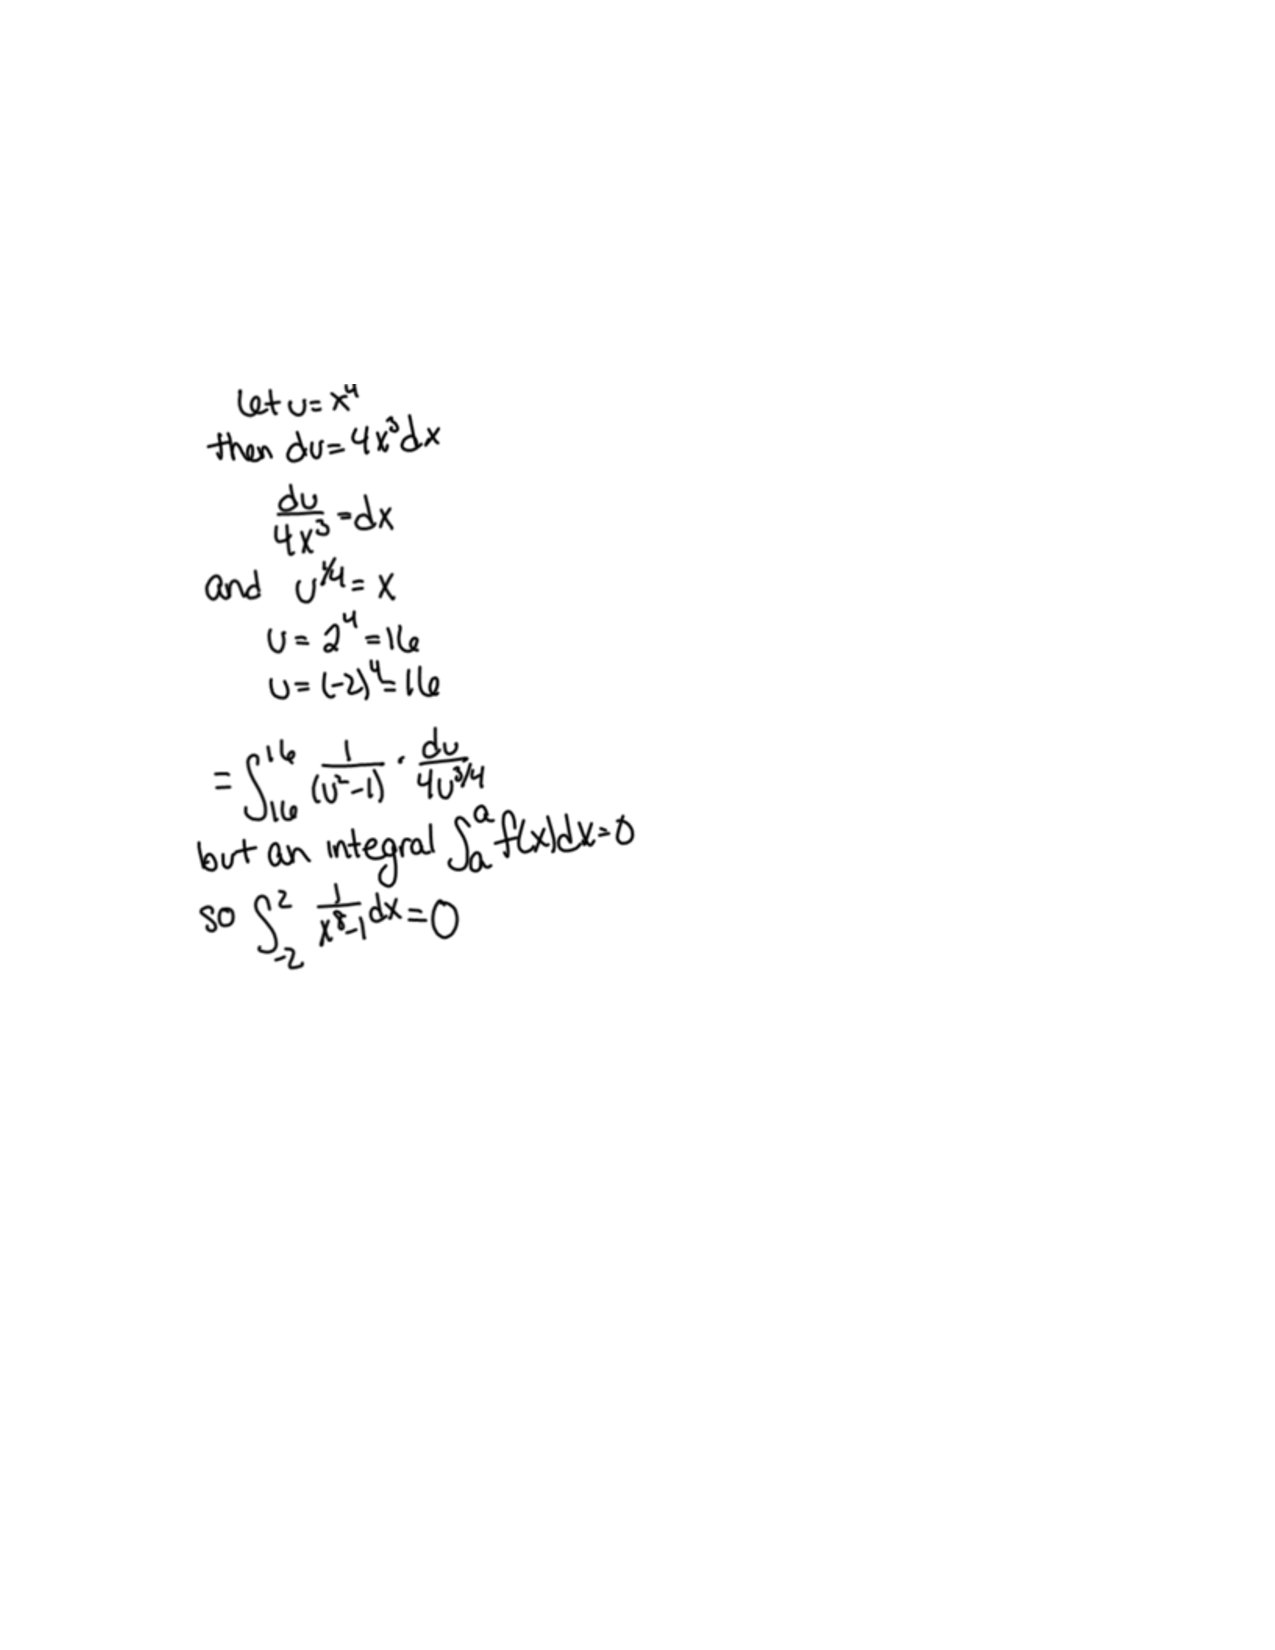
\includegraphics[trim= 170 420 250 180]{Figure1.pdf}
%\end{image}

%add a ``.'' below when used in a specific directory.
\newcommand{\RR}{\mathbb R}
\renewcommand{\d}{\,d}
\newcommand{\dd}[2][]{\frac{d #1}{d #2}}
\renewcommand{\l}{\ell}
\newcommand{\ddx}{\frac{d}{dx}}
\newcommand{\dfn}{\textbf}
\newcommand{\eval}[1]{\bigg[ #1 \bigg]}

\usepackage{multicol}

\renewenvironment{freeResponse}{
\ifhandout\setbox0\vbox\bgroup\else
\begin{trivlist}\item[\hskip \labelsep\bfseries Solution:\hspace{2ex}]
\fi}
{\ifhandout\egroup\else
\end{trivlist}
\fi} %% we can turn off input when making a master document

\title{Calculus in polar coordinates}  

\begin{document}
\begin{abstract}		\end{abstract}
\maketitle



\section{Warm up:}
\begin{enumerate}
\item True or False:  The slope of the tangent line to the curve $r = f(\theta)$ at the point $(r_0, \theta_0)$ is given by $f'(\theta_0)$.  

\item True or False: The area enclosed by the curve $r=2\cos(\theta)$ is 
$$\int_{0}^{2\pi} \frac{1}{2} (2 \cos (\theta))^2 d \theta = \int_0^{2\pi} 1+\cos(2\theta) d\theta = 2\pi.$$
\end{enumerate}

	\begin{freeResponse}
\begin{enumerate}
\item	{\bf False.}  The slope of the tangent line to the curve $r = f(\theta)$ at $(r_0, \theta_0)$ is given by
		\[
		\frac{\d y}{\d x} = \frac{f'(\theta_0) \sin \theta_0 + f(\theta_0) \cos \theta_0}{f'(\theta_0) \cos \theta_0 - f(\theta_0) \sin \theta_0 } \neq f'(\theta_0).
		\]

\item {\bf False.} The curve $r=\cos(\theta)$ is a circle of radius 1 centered at (1,0). The curve traces out the circle \textcolor{red}{twice} for $\theta$ in $[0, 2\pi]$. So the area enclosed is just $\int_0^{\pi} \frac{1}{2} (2 \cos(\theta))^2 d\theta = \pi$.
\end{enumerate}
	\end{freeResponse}
	
\begin{instructorNotes}
The point of $b$ is for the students to realize that you need to think about the curve before blindly using a formula.
\end{instructorNotes}







\section{Group work:}



%problem 1
\begin{problem}
Find the equation of the tangent line to $r = 2 - \sin \theta$ at $\theta = \frac{\pi}{3}$.  
Also, determine for what values of $\theta$ the tangent lines to the curve are vertical or horizontal.
	\begin{freeResponse}
	We use the formula from the warm-up to find $\frac{\d y}{\d x}$ when $f(\theta) = 2 - \sin \theta$:
		\begin{align*}
		\frac{\d y}{\d x}
		&= \frac{f'(\theta) \sin \theta + f(\theta) \cos \theta}{f'(\theta) \cos \theta - f(\theta) \sin \theta } \\
		&= \frac{(- \cos \theta)(\sin \theta) + (2 - \sin \theta)(\cos \theta)}{(-\cos \theta)(\cos \theta) - (2 - \sin \theta)(\sin \theta)}.
		\end{align*}
	So
		\begin{align*}
		\eval{\frac{\d y}{\d x}}_{\theta = \frac{\pi}{3}} 
		&= \frac{(- \cos \frac{\pi}{3})(\sin \frac{\pi}{3}) + (2 - \sin \frac{\pi}{3})(\cos \frac{\pi}{3})}{(-\cos \frac{\pi}{3})(\cos \frac{\pi}{3}) - (2 - \sin \frac{\pi}{3})(\sin \frac{\pi}{3})}  \\
		&= \frac{\left( - \frac{1}{2} \cdot \frac{\sqrt{3}}{2} \right) + \left( 2 - \frac{\sqrt{3}}{2} \right) \left( \frac{1}{2} \right)}{\left( - \frac{1}{2} \cdot \frac{1}{2} \right) - \left( 2 - \frac{\sqrt{3}}{2} \right) \left( \frac{\sqrt{3}}{2} \right)}  \\
		&= \frac{- \sqrt{3} + 4 - \sqrt{3}}{-1 - 4 \sqrt{3} + 3}  \\
		&= \frac{4 - 2 \sqrt{3}}{2 - 4 \sqrt{3}}  \\
		&= \frac{2 - \sqrt{3}}{1 - 2 \sqrt{3}}.
		\end{align*}
	Also, when $\theta = \frac{\pi}{3}$, $r = 2 - \frac{\sqrt{3}}{2} = \frac{4 - \sqrt{3}}{2}$.  
	Therefore
		\begin{align*}
		&x = r \cos \theta = \frac{4 - \sqrt{3}}{2} \cdot \frac{1}{2} = 1 - \frac{\sqrt{3}}{4}  \\
		&y = r \sin \theta = \frac{4 - \sqrt{3}}{2} \cdot \frac{\sqrt{3}}{2} = \sqrt{3} - \frac{3}{4}.
		\end{align*}
	Thus, the equation of the tangent line when $\theta = \frac{\pi}{3}$ is
		\[
		\boxed{y - \left( \sqrt{3} - \frac{3}{4} \right) = \frac{2 - \sqrt{3}}{1 - 2 \sqrt{3}} \left( x - \left( 1 - \frac{\sqrt{3}}{4} \right) \right)}
		\]
		
	To find all vertical and horizontal tangent lines, we need to find where the numerator and denominator of $\frac{\d y}{\d x}$ are equal to $0$.
	
	{\bf Numerator:}
		\begin{align*}
		(- \cos \theta)(\sin \theta) + (2 - \sin \theta)(\cos \theta) &= 0  \\
		- \sin \theta \cos \theta + 2 \cos \theta - \sin \theta \cos \theta &= 0  \\
		2 \cos \theta - 2 \sin \theta \cos \theta &= 0  \\
		2 \cos \theta (1 - \sin \theta) &= 0  \\
		\cos \theta = 0 \quad \text{or} \quad \sin \theta &= 1  \\
		\theta = \frac{\pi}{2} + k \pi  \quad  \text{or}  \quad  \theta &= \frac{\pi}{2} + 2k\pi \quad \text{for } k \text{ an integer}  \\
		\theta = \frac{\pi}{2} + k \pi  &\quad \text{for } k \text{ an integer}
		\end{align*}
		
	{\bf Denominator:}
		\begin{align*}
		(-\cos \theta)(\cos \theta) - (2 - \sin \theta)(\sin \theta) &= 0  \\
		- \cos^2 \theta - 2 \sin \theta + \sin^2 \theta &= 0  \\
		-1 + \sin^2 \theta - 2 \sin \theta + \sin^2 \theta &= 0  \\
		2 \sin^2 \theta - 2 \sin \theta - 1 &= 0  \\
		\sin \theta &= \frac{2 \pm \sqrt{4 + 8}}{4}  	\quad  {\color{red}\text{throw away the ``+'' }}\\
		\sin \theta &= \frac{1 - \sqrt{3}}{2}  \quad {\color{red}\text{since it is out of the range of sin}}\\
		\theta &= \sin^{-1} \left( \frac{1-\sqrt{3}}{2} \right) + 2 k \pi 	\quad \text{for k an integer}
		\end{align*}
	Note that $\sin \theta = \frac{1-\sqrt{3}}{2}$ twice during a period. The other one occurs at $\pi - \sin^{-1}\left(\frac{1-\sqrt{3}}{2}\right)$. 
		
	Then, since these two collections of angles are disjoint, the horizontal tangent lines occur when
		\[
		\boxed{\theta = \frac{\pi}{2} + k \pi}  \quad \text{for } k \text{ an integer}
		\]
	and the vertical tangent lines occur when
		\[
		\boxed{\theta = \sin^{-1} \left( \frac{1-\sqrt{3}}{2} \right) + 2 k \pi, \theta = \pi - \sin^{-1}\left(\frac{1-\sqrt{3}}{2}\right)+2k \pi} 	\quad \text{for k an integer}
		\]
	\end{freeResponse}
	
\end{problem}

\begin{instructorNotes}
They probably haven't seen how to find the other angle for which $\sin \theta = \frac{1-\sqrt{3}}{2}$ since Pre-Calculus. 
\end{instructorNotes}







%problem 2
\begin{problem}
Graph each region and then SET UP an integral for the area of the region:
	\begin{enumerate}
	\item  Outside the small loop and inside the large loop of $r = 3 - 6 \sin \theta$.
	\item  Inside both of the curves $r = 4 \cos \theta$ and $r = 1 - \cos \theta$.
	\end{enumerate} 
	{\it Note that you do not need to evaluate these integrals.}
	
	\begin{image}
	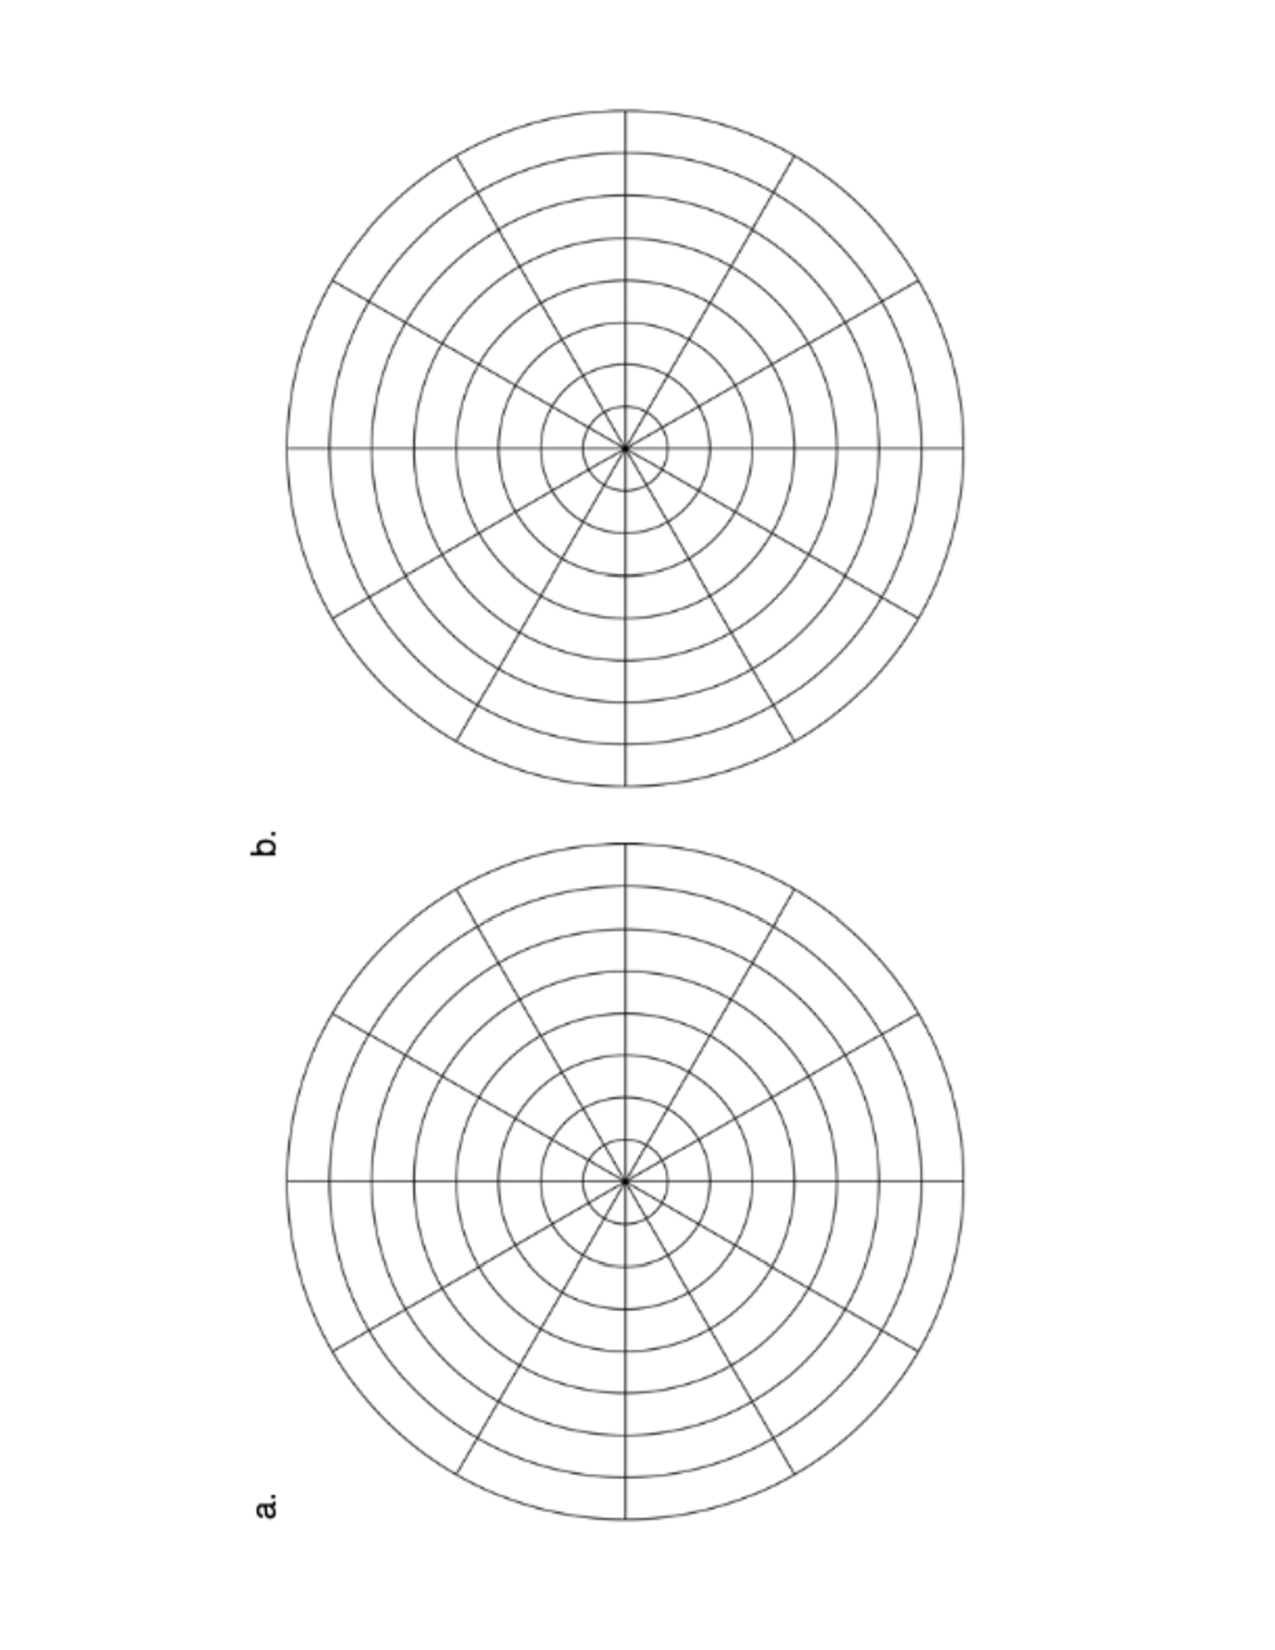
\includegraphics[angle=-89.99,trim= 120 220 140 220, scale=0.6]{Figure11-3-1.pdf}
	\end{image}
	
	\begin{freeResponse}
	\begin{enumerate}
	\item  The graph of the region is given below.
	
		\begin{image}
		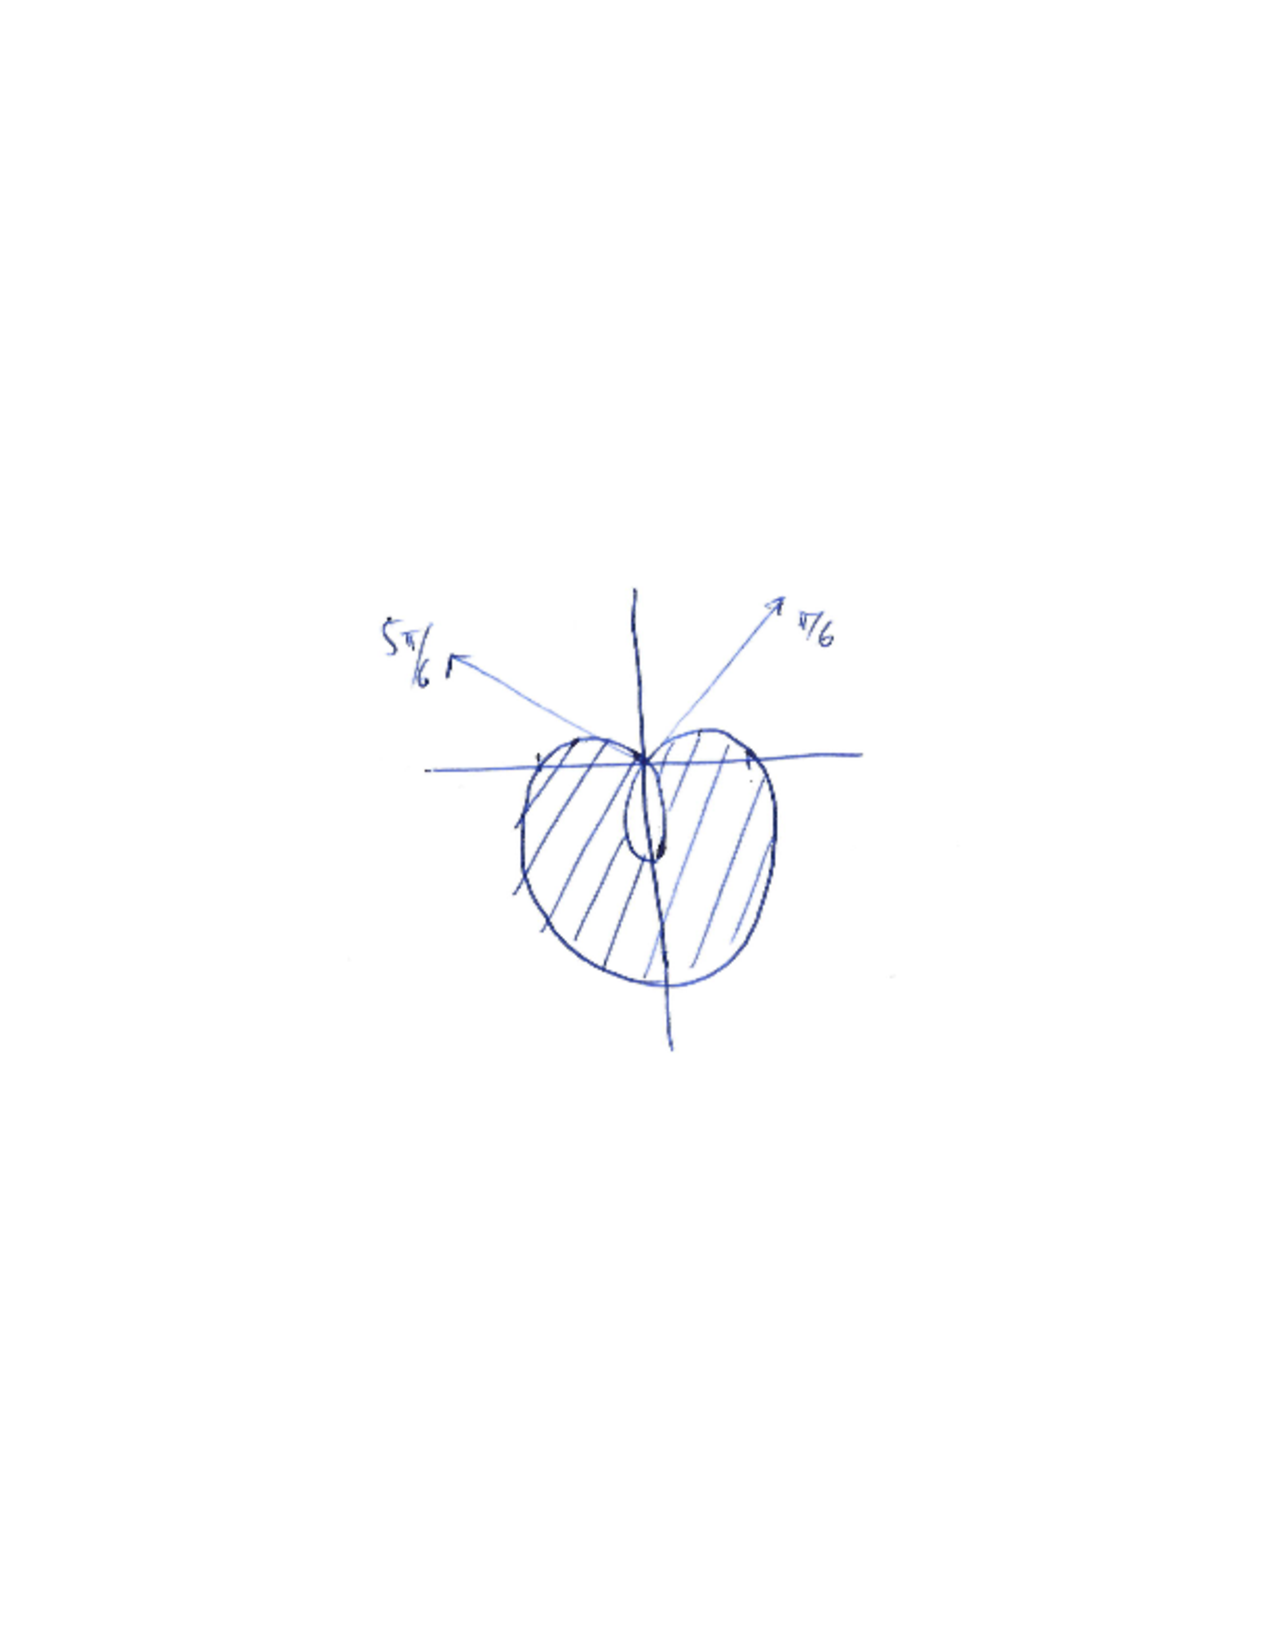
\includegraphics[trim= 280 280 170 280, scale=0.6]{Figure11-3-2.pdf}
		\end{image}
		
	To find the area inside the smaller loop, we need to first find the values of $\theta$ for which $r = 0$.
	So we compute
		\begin{align*}
		&3 - 6 \sin \theta = 0  \\
		\Longrightarrow \qquad &\sin \theta = \frac{1}{2}  \\
		\Longrightarrow \qquad &\theta = \frac{\pi}{6}, \frac{5 \pi}{6}.
		\end{align*}
	Hence, the area of the smaller loop is
		\[
		\frac{1}{2} \int_{\frac{\pi}{6}}^{\frac{5 \pi}{6}} (3 - 6 \sin \theta)^2 \d \theta.
		\]
		
	To find the area of the outer loop, we just integrate over the other values of $\theta$:
		\[
		\frac{1}{2} \int_0^{\frac{\pi}{6}} (3 - 6 \sin \theta)^2 \d \theta
		+ \frac{1}{2} \int_{\frac{5 \pi}{6}}^{2 \pi} (3 - 6 \sin \theta)^2 \d \theta.
		\]
		
	Therefore, the area of the region inside the outer loop and outside the inner loop is
		\[
		\boxed{\frac{1}{2} \left[ \int_0^{\frac{\pi}{6}} (3 - 6 \sin \theta)^2 \d \theta - \int_{\frac{\pi}{6}}^{\frac{5 \pi}{6}} (3 - 6 \sin \theta)^2 \d \theta + \int_{\frac{5 \pi}{6}}^{2 \pi} (3 - 6 \sin \theta)^2 \d \theta \right]    }
		\]
		
		
	
	\item  We first graph $r = 4 \cos \theta$.
		\begin{image}
		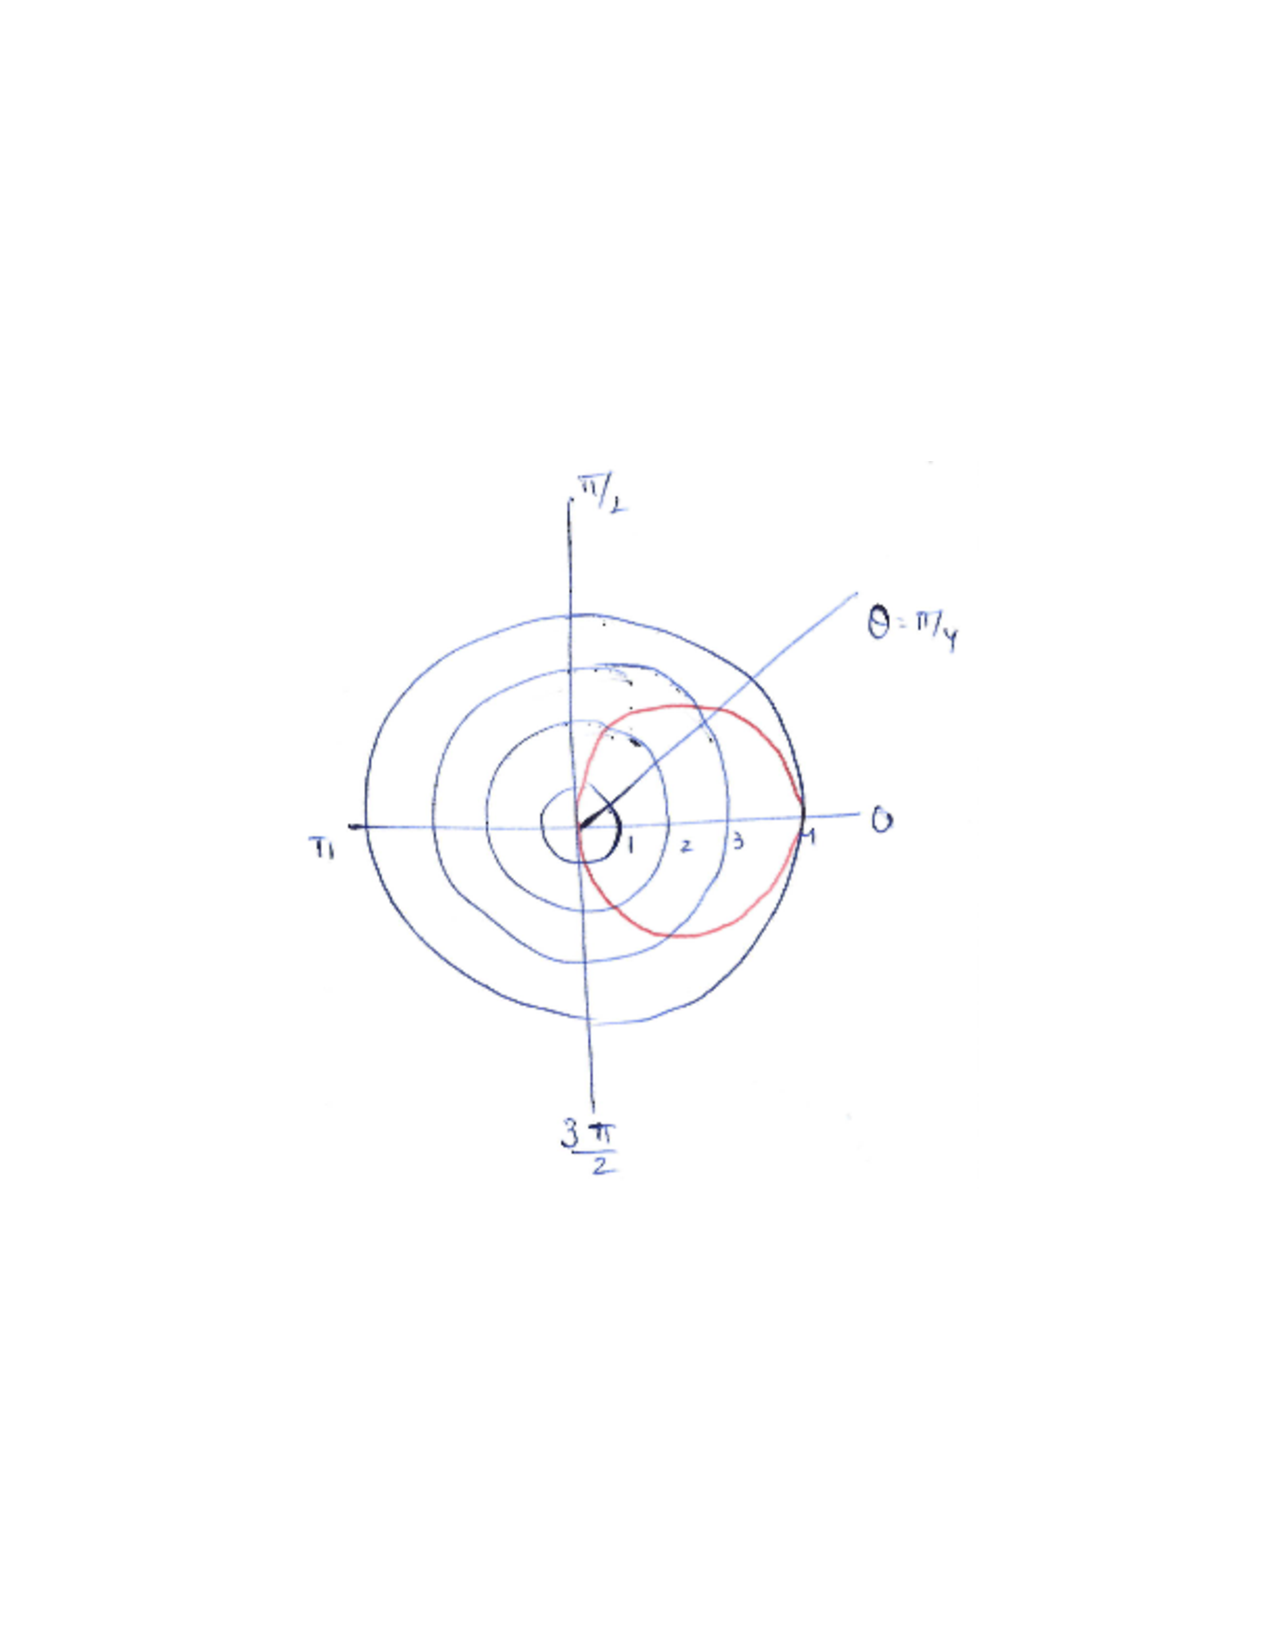
\includegraphics[trim= 170 220 170 230, scale=0.6]{Figure11-3-3.pdf}
		\end{image}
		
	Now we graph $r = 1 - \cos \theta$
		\begin{image}
		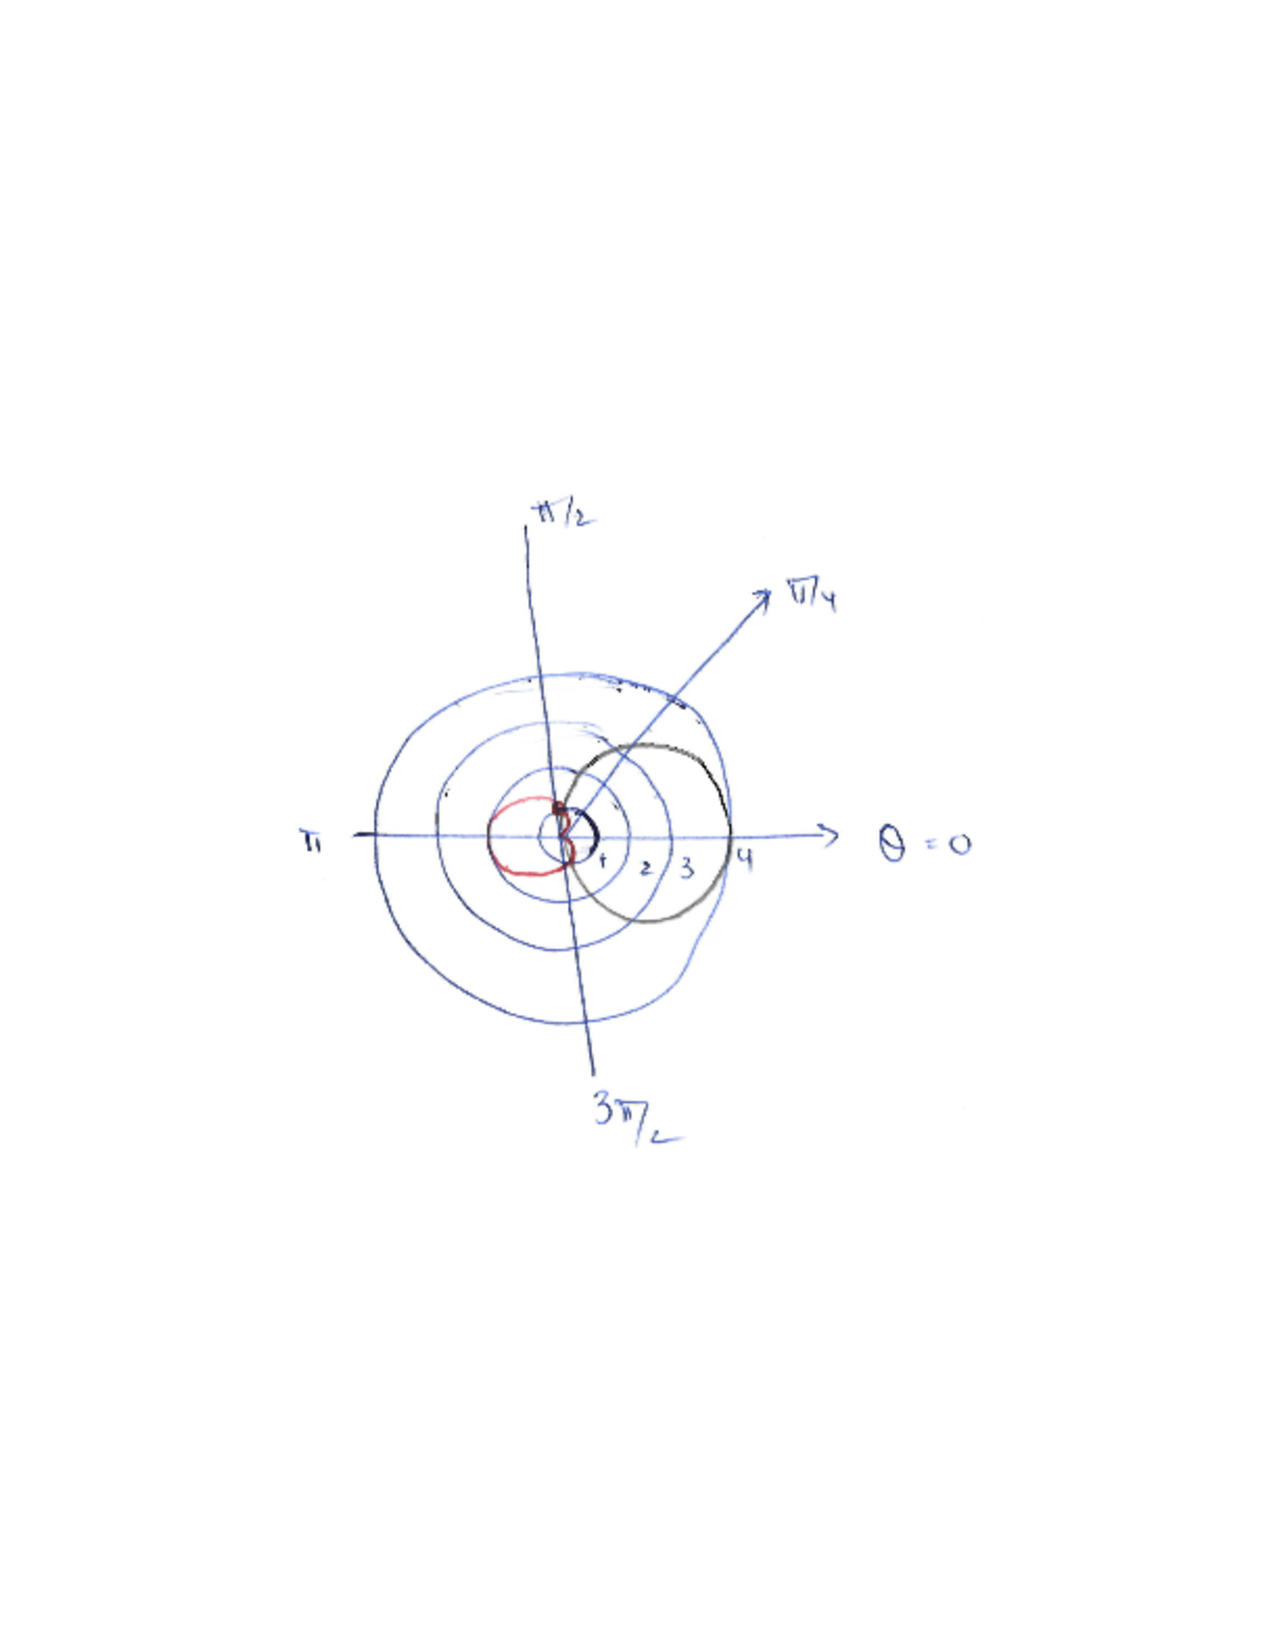
\includegraphics[trim= 170 240 170 230, scale=0.6]{Figure11-3-4.pdf}
		\end{image}
		
	Here are the two graphs in the same picture
		\begin{image}
		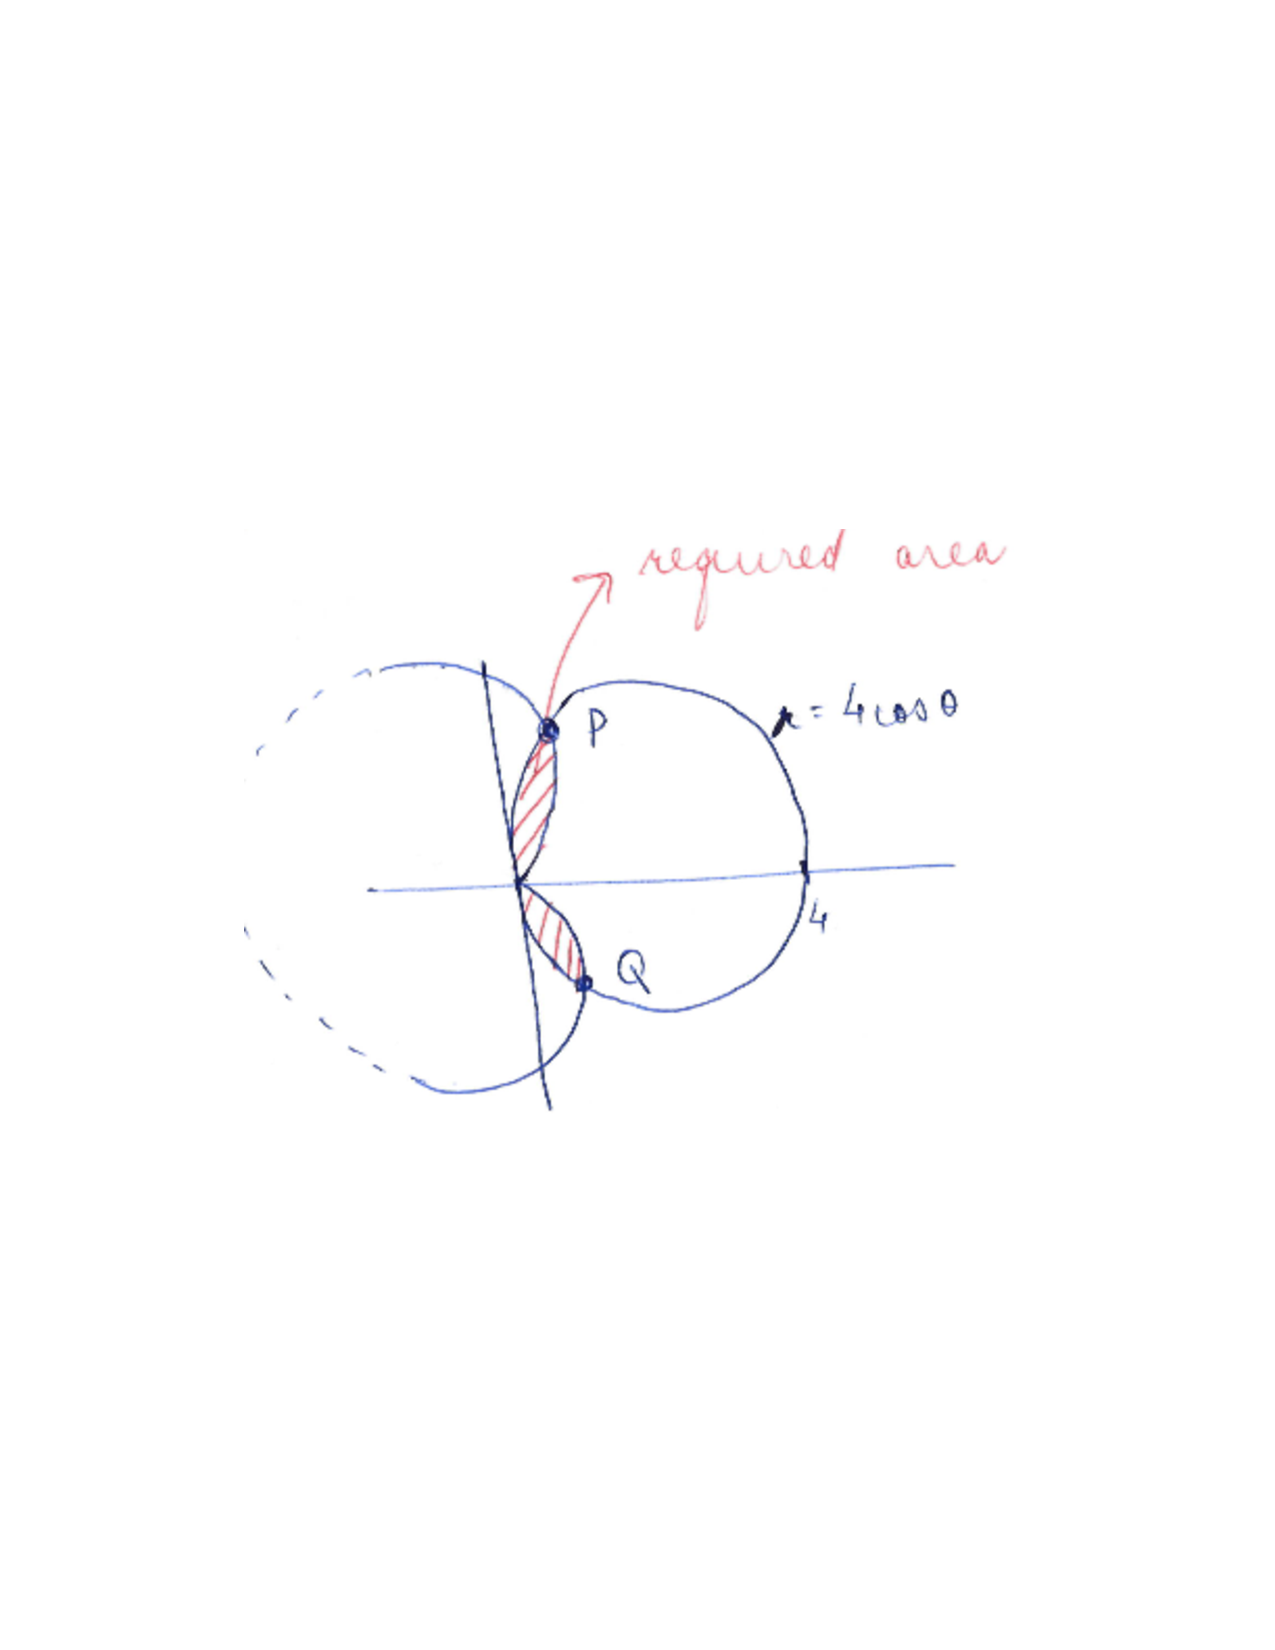
\includegraphics[trim= 170 240 170 230, scale=0.6]{Figure11-3-5.pdf}
		\end{image}
		
	To find the points where the two curves intersect, we solve
		\begin{align*}
		4 \cos \theta &= 1 - \cos \theta  \\
		5 \cos \theta &= 1  \\
		\cos \theta &= \frac{1}{5}  \\
		\theta &= \pm \cos^{-1} \left( \frac{1}{5} \right) := \theta_0.
		\end{align*}
	Using the symmetry of the graph we find the area of one leaf and then double it.  
	Therefore, the area between the curves is
		\[
		\boxed{ 2 \left[ \frac{1}{2} \int_0^{\theta_0} (1 - \cos \theta)^2 \d \theta + \frac{1}{2} \int_{\theta_0}^{\frac{\pi}{2}} (4 \cos \theta)^2 \d \theta \right] }
		\]
	In the following picture, the left-hand integral is (1) and the right-hand integral is (2).
		\begin{image}
		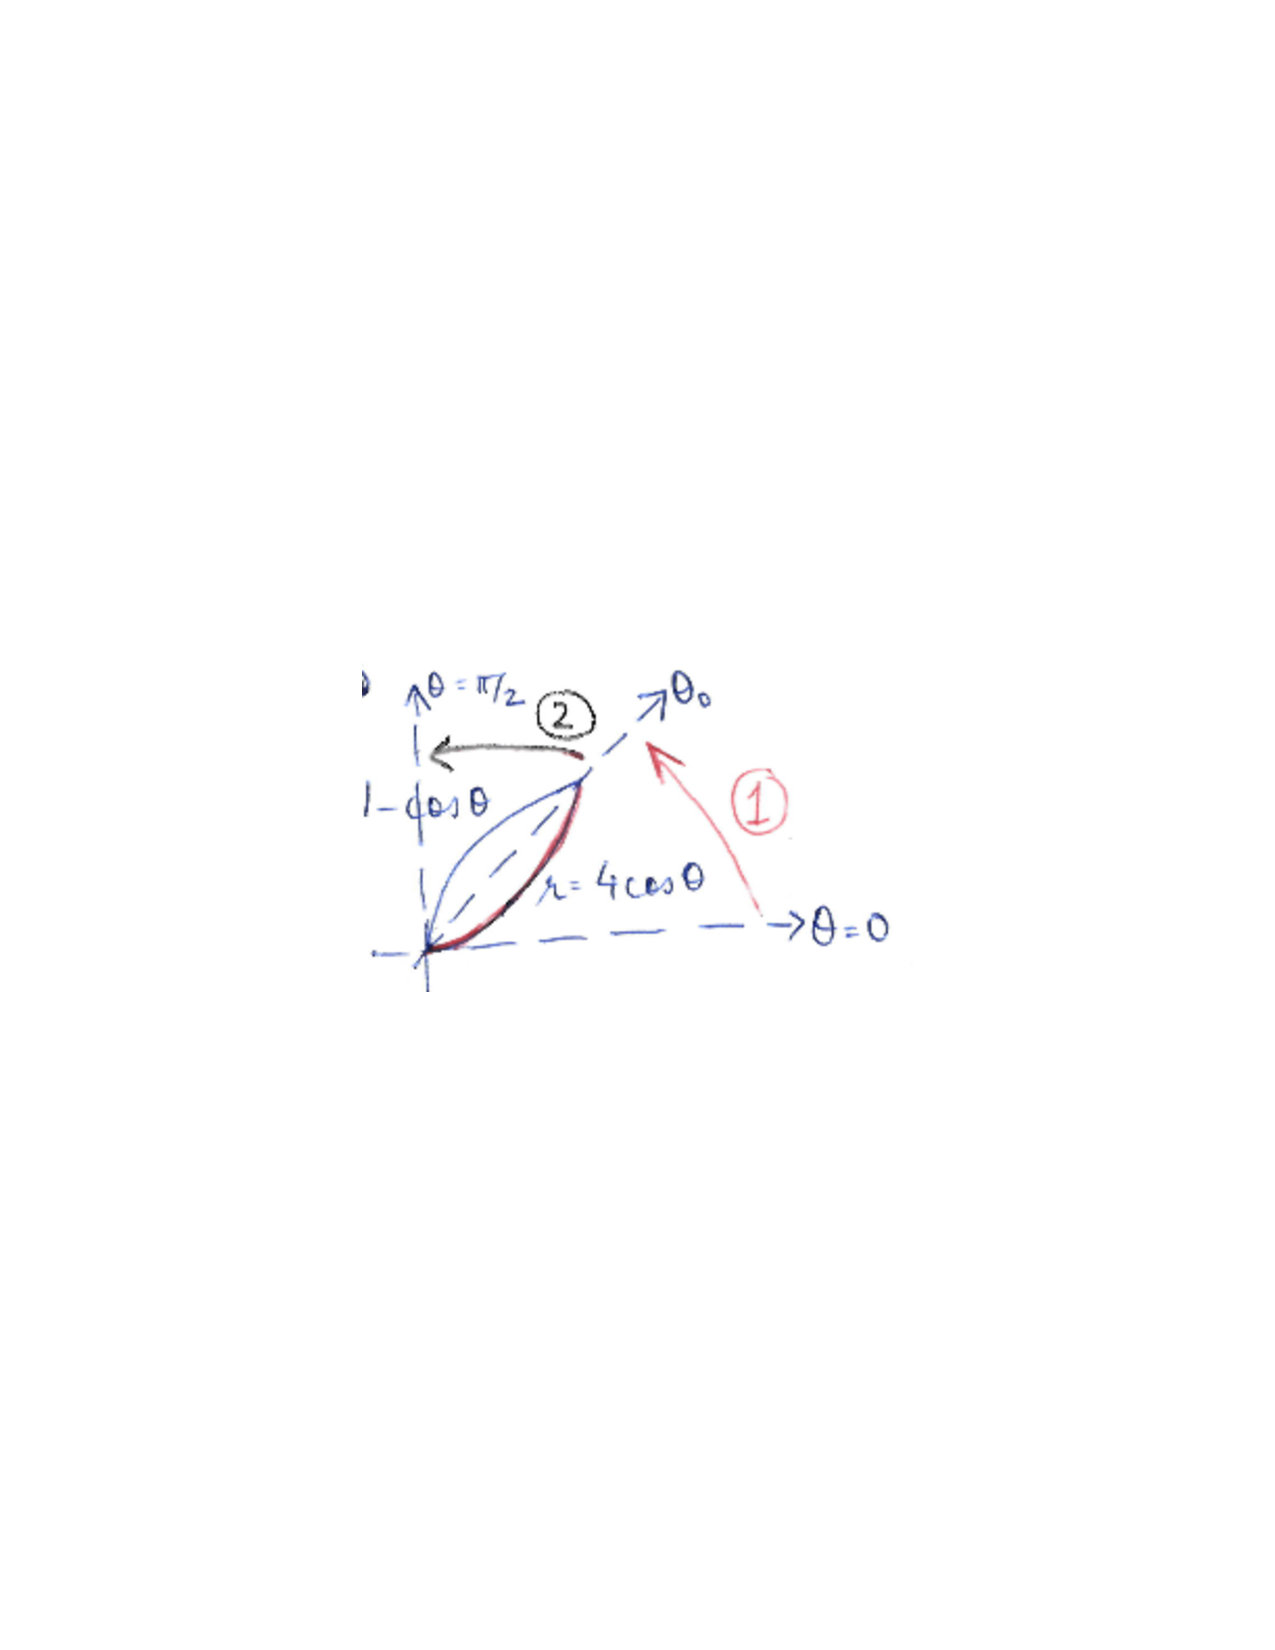
\includegraphics[trim= 170 320 170 310, scale=0.8]{Figure11-3-6.pdf}
		\end{image}
	
	\end{enumerate}
	\end{freeResponse}
		
\end{problem}

\begin{instructorNotes}
If you have time at the end, you can go over how you would evaluate these integrals. 
\end{instructorNotes}




\begin{comment}
%problem 3
\begin{problem}

	\begin{freeResponse}
	
	\end{freeResponse}

\end{problem}

\begin{instructorNotes}

\end{instructorNotes}
\end{comment}
















	
	
	
	
	
	
	
	
	

	










								
				
				
	














\end{document} 


















